%!TEX program = xelatex
\documentclass[11pt,a4paper]{article}

% --- fonts / Chinese for author name only ---
\usepackage[UTF8,scheme=plain]{ctex}
\usepackage{fontspec}
\setmainfont{TeX Gyre Termes}
\setmonofont{Latin Modern Mono}[Scale=0.92]

% --- core ---
\usepackage{amsmath,amssymb,bm}
\usepackage{booktabs,tabularx,array,multirow}
\usepackage{graphicx}
\usepackage{subcaption}
\usepackage{float}
\usepackage{natbib}
\usepackage{xcolor}
\usepackage[margin=2.5cm]{geometry}
\usepackage{hyperref}
\usepackage{setspace}
\onehalfspacing
\usepackage{caption}
\captionsetup{font=small,labelfont=bf,skip=6pt}

\hypersetup{colorlinks=true,linkcolor=black,citecolor=black,urlcolor=black}

\newcolumntype{L}{>{\raggedright\arraybackslash}X}
\newcolumntype{C}{>{\centering\arraybackslash}X}

\title{G1 Locomotion}
\author{
  \begin{tabular}{c}
    李子墨 \\
    \small 学号 241098038 \\
    \small \texttt{3234454007@qq.com}
  \end{tabular}
}
\date{}

\begin{document}
\maketitle

\begin{abstract}

I trained a velocity-tracking policy with PPO for the Unitree G1 humanoid and adapted it to achieve goal-tracking behavior.
In addition, I experimented with two out-of-distribution (OOD) scenarios for the policy---OOD speed and OOD terrain---and then fine-tuned the policy to overcome the OOD failures.

\end{abstract}

\section{Introduction}

The goal is to make Unitree G1 walk to a target in Isaac Lab. I solve this in
two steps.

\textbf{Training:} I use PPO to train a velocity-tracking policy. Its command is
$(v_x,v_y,\omega_z)$, where $v_x$ is forward speed, $v_y$ is lateral speed, and
$\omega_z$ is turning speed.

\textbf{Inference:} I keep the trained policy fixed. A simple proportional
controller converts the relative goal position into a velocity command. The
policy then follows that command to reach the goal.

I also test the policy in two situations outside its training distribution:
\begin{itemize}
  \item \textbf{Faster commands:} the base policy is trained with
  $v_x\in[0,1]\,\mathrm{m/s}$ and tested at speeds up to
  $2\,\mathrm{m/s}$.
  \item \textbf{Rough terrain:} the flat-ground policy is tested and
  fine-tuned on stairs, boxes, slopes, and height noise.
\end{itemize}

In the recorded tests, the base policy falls at
$v_x=1.4\,\mathrm{m/s}$, while the fine-tuned policy walks at
$2\,\mathrm{m/s}$. After a short rough-terrain fine-tune, the policy
also walks over the tested uneven surfaces without a height scan.

\section{Related Work}
\label{sec:related}

\paragraph{Bipedal locomotion.}
Classical biped controllers often use simplified models such as
SLIP~\citep{blickhan1989slip}, LIP~\citep{kajita2001lip}, and
ZMP~\citep{vukobratovic2004zmp} to plan stable motion. These methods model balance
directly but require carefully designed controllers.

\paragraph{Learning locomotion.}
Deep reinforcement learning can learn locomotion directly from simulated
experience. With thousands of environments running in parallel, a
velocity-tracking policy can be trained efficiently~\citep{rudin2022legged}.
I follow that approach for G1.

\paragraph{Training tools.}
PPO is an actor--critic algorithm that limits each policy update with a clipped
objective~\citep{schulman2017ppo}. I use PPO from RSL-RL, Isaac Sim for
GPU-parallel physics, and Isaac Lab for the G1 robot and locomotion
environment.

\section{Training}
\label{sec:train}

I simulate Unitree G1 in Isaac Lab and train a velocity-tracking policy with PPO (RSL-RL).
4096 environments run in parallel on GPU; each step the policy outputs joint targets, physics advances, and rewards are collected for the update.
The policy follows a randomly sampled command $\mathbf{c}_t = (v_x, v_y, \omega_z)$.

\subsection{MDP}

The learning objective is to make G1 follow a commanded planar velocity
$\mathbf{c}_t=(v_x,v_y,\omega_z)$. I use the official flat-ground task
\texttt{G1FlatEnvCfg} and disable its height scanner. One control step proceeds
as follows: the policy observes the robot and the current command, outputs a
target offset for every actuated joint, and then the simulator advances the
physics and evaluates how well the resulting motion follows the command.

Formally, the simulator state $s_t$ contains the complete physical state of the
robot and environment. The policy does not receive $s_t$ directly; it receives
the 123-dimensional observation
\[
\mathbf{o}_t =
\left[
\mathbf{v}^{b}_t,\,
\boldsymbol{\omega}^{b}_t,\,
\mathbf{g}^{b}_t,\,
\mathbf{c}_t,\,
\mathbf{q}_t-\mathbf{q}_{0},\,
\dot{\mathbf{q}}_t,\,
\mathbf{a}_{t-1}
\right],
\qquad \mathbf{o}_t\in\mathbb{R}^{123}.
\]
Here, $\mathbf{v}^{b}_t$ and $\boldsymbol{\omega}^{b}_t$ are the base linear
and angular velocities (3 values each), $\mathbf{g}^{b}_t$ is the gravity
direction expressed in the base frame (3), and $\mathbf{c}_t$ is the velocity
command (3). The remaining terms are the 37 joint positions relative to the
default pose, the 37 joint velocities, and the previous 37-dimensional action.
These dimensions sum to $3+3+3+3+37+37+37=123$. Small uniform noise is added
to the body and joint measurements during training. Because the height scanner
is disabled, the policy receives no direct description of the terrain.

\paragraph{Action and transition.}
The action $\mathbf{a}_t\in\mathbb{R}^{37}$ does not specify joint torque
directly. Instead, each component is a position offset from the default pose:
\[
\mathbf{q}^{\mathrm{target}}_t
=\mathbf{q}_{0}+0.5\,\mathbf{a}_t.
\]
The joint controllers track these targets while Isaac Sim advances the robot
dynamics from $s_t$ to $s_{t+1}$. Including $\mathbf{a}_{t-1}$ in the next
observation lets the policy account for its previous target when producing a
smooth action sequence.

\paragraph{Reward and termination.}
The reward is the weighted sum supplied by the official G1 flat task. Its
largest positive terms reward tracking the commanded XY velocity and yaw rate
(weight $+1.0$ each). A feet-air-time term ($+0.75$) encourages stepping.
Penalties discourage foot sliding ($-0.1$), body tilt ($-1.0$), vertical
velocity ($-0.2$), roll and pitch angular velocity ($-0.05$), and joint
deviation or limit violations (weights from $-1.0$ to $-0.05$). Smaller
regularizers penalize rapid action changes
($-5{\times}10^{-3}$), joint torques ($-2{\times}10^{-6}$), and joint
accelerations ($-1{\times}10^{-7}$). Termination incurs a reward of $-200$.
Thus, maximizing return asks the robot to follow the command while maintaining
a stable, smooth, physically plausible gait.

\paragraph{PPO configuration.}
The actor and critic use MLPs with hidden layers $[256,128,128]$. PPO collects
24 steps from each of 4096 parallel environments per iteration, with clipping
parameter $0.2$, discount $\gamma=0.99$, GAE parameter $\lambda=0.95$, and
entropy coefficient $0.008$.

\subsection{Velocity-policy training}

I train one policy to follow randomly sampled velocity commands on flat ground.
The command ranges are
\[
v_x \in [0, 1]\,\mathrm{m/s},\quad
v_y \in [-0.5, 0.5]\,\mathrm{m/s},\quad
\omega_z \in [-1, 1]\,\mathrm{rad/s},
\]
where $v_x$ controls forward motion, $v_y$ controls lateral motion, and
$\omega_z$ controls turning. A small fraction of environments receive the
standing command $\mathbf{c}_t=\mathbf{0}$, so the same policy also learns to
remain still. Training runs for 1750 iterations.
Figure~\ref{fig:tb-base} shows the mean reward rising steadily while the
velocity-tracking errors fall, and Figure~\ref{fig:train} shows the resulting
gait on flat ground.

\begin{figure}[H]
\centering
\begin{subfigure}[t]{0.33\textwidth}
\centering
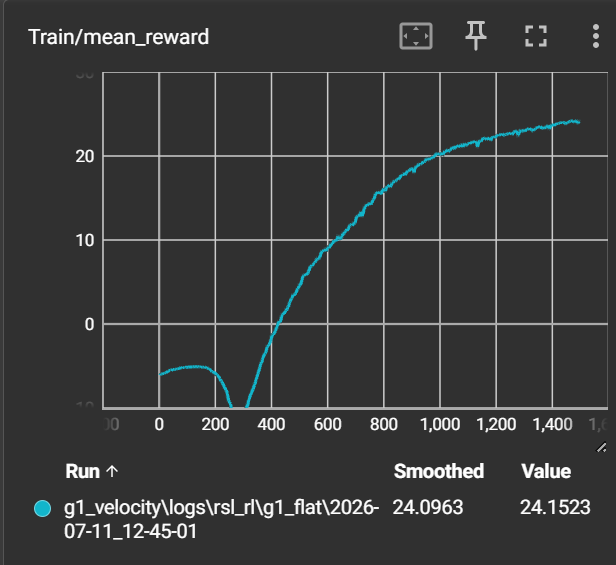
\includegraphics[width=\linewidth]{figures/tb-g1_velocity_mean_reward.png}
\caption*{Mean reward.}
\end{subfigure}
\hfill
\begin{subfigure}[t]{0.66\textwidth}
\centering
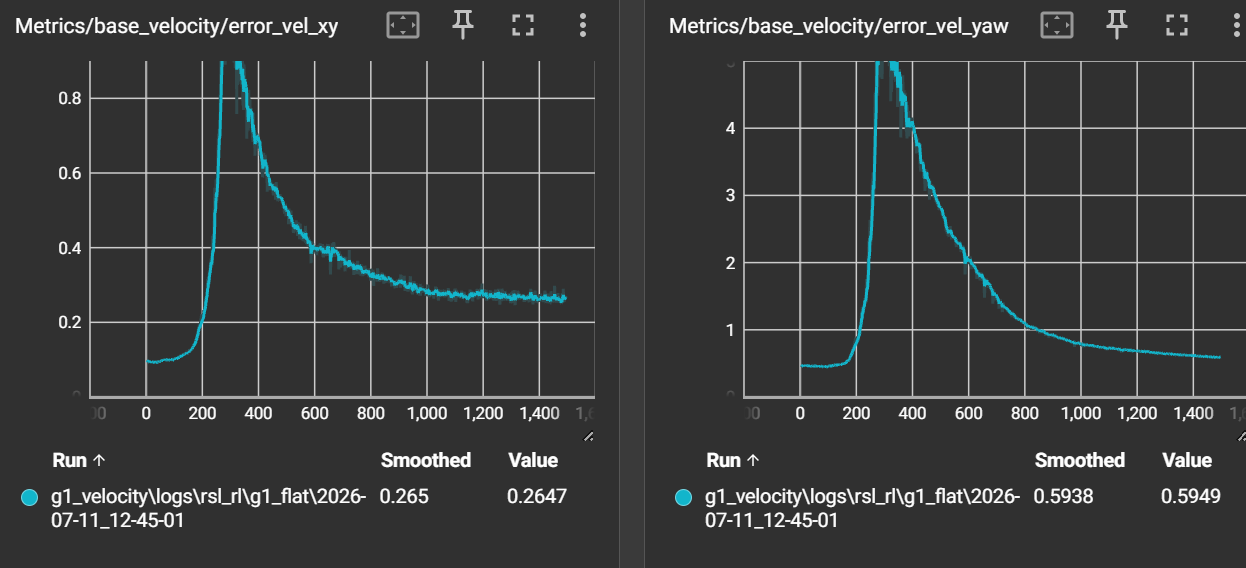
\includegraphics[width=\linewidth]{figures/tb_g1_velocity_metrics_error.png}
\caption*{Velocity tracking errors.}
\end{subfigure}
\caption{Base velocity-policy training curves.}
\label{fig:tb-base}
\end{figure}

\begin{figure}[H]
\centering
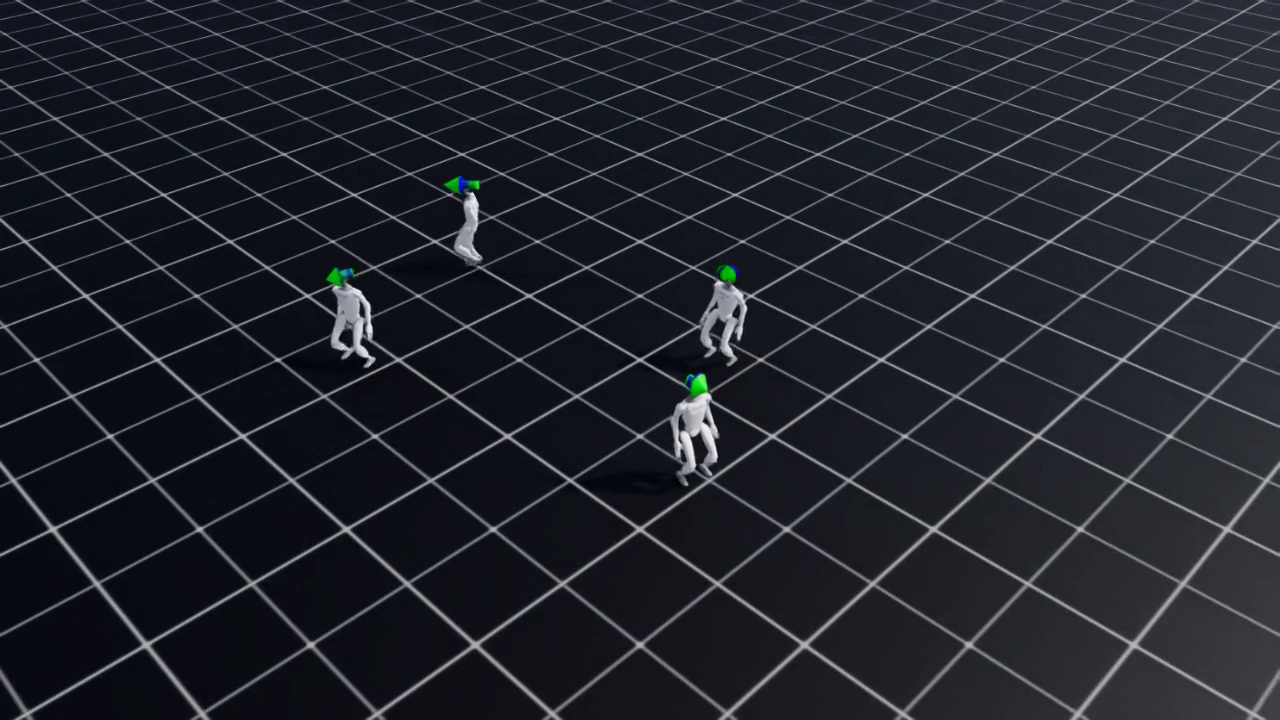
\includegraphics[width=0.72\textwidth]{figures/fig_flat.png}
\caption{Trained velocity-tracking policy on flat ground (random commands).}
\label{fig:train}
\end{figure}

\section{Inference}
\label{sec:inference}

At inference, I freeze the policy weights and use a proportional controller to
convert the goal displacement into $(v_x,v_y,\omega_z)$. The policy follows
these commands with the same observation and action spaces used during
training.

\paragraph{Goal-to-velocity controller.}
At every control step, the world-frame goal is expressed in the robot's yaw
frame as $(d_x,d_y)$. The angle
$\psi=\mathrm{atan2}(d_y,d_x)$ is the direction from the robot to the goal in
that frame. The velocity command is then computed as follows:
\begin{enumerate}
  \item If $\sqrt{d_x^2+d_y^2}<0.35\,\mathrm{m}$, set
  $\mathbf{c}_t=\mathbf{0}$ so that the robot stands near the goal.
  \item Otherwise, apply proportional control:
  \[
  v_x = \mathrm{clip}(k_\ell d_x,\, 0,\, 1),\quad
  v_y = \mathrm{clip}(k_\ell d_y,\, -0.5,\, 0.5),\quad
  \omega_z = \mathrm{clip}(k_a \psi,\, -1,\, 1),
  \]
  with $k_\ell = 1.0$ and $k_a = 1.5$.
\end{enumerate}
Clipping keeps every command within the ranges seen during training. In
particular, the controller never requests backward motion; when a goal is
behind the robot, yaw control turns the robot toward it before substantial
forward motion is commanded.

\paragraph{Result.}
In the recorded simulation, the frozen policy walks toward the marked goal and
stands after entering the $0.35\,\mathrm{m}$ stopping region
(Figure~\ref{fig:inference}).

\begin{figure}[H]
\centering
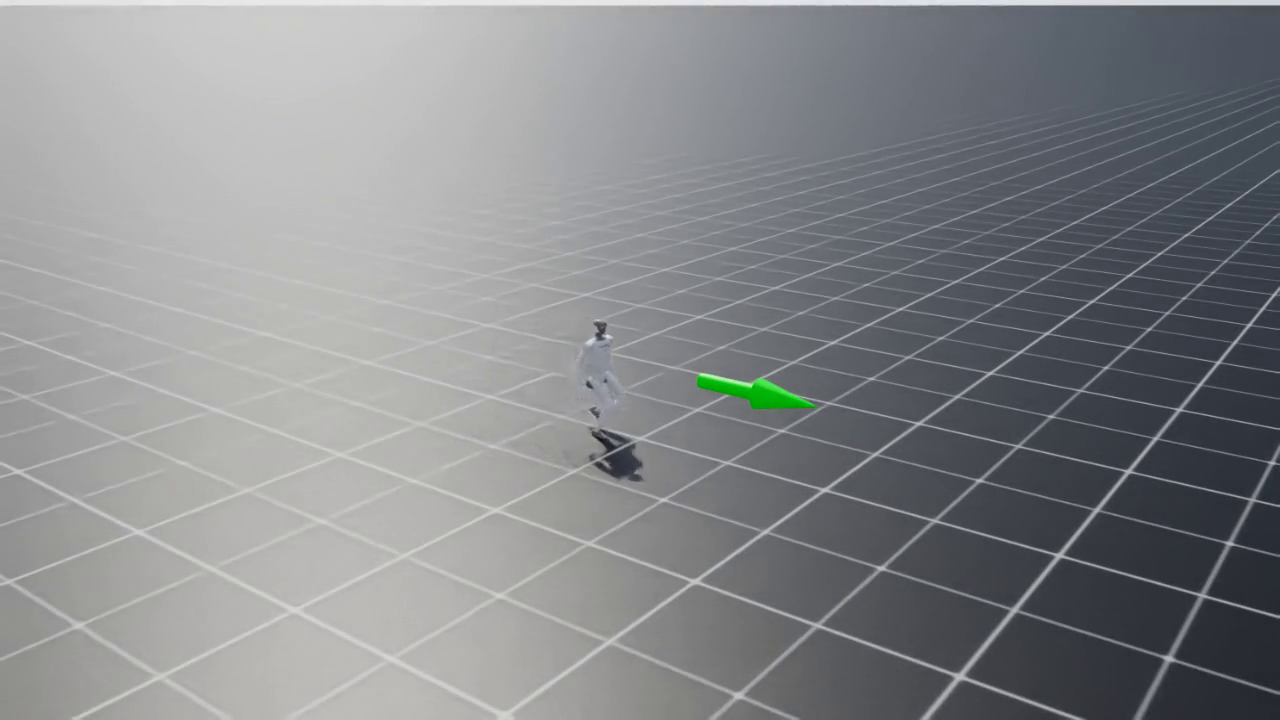
\includegraphics[width=0.72\textwidth]{figures/fig_goal.png}
\caption{Goal-directed inference. The proportional controller steers the
frozen velocity policy toward the green marker.}
\label{fig:inference}
\end{figure}

\section{Exploratory Experiment I: Forward-Speed Generalization}
\label{sec:ood}

The base policy was trained with forward commands no greater than
$1\,\mathrm{m/s}$. This experiment asks what happens when it receives a faster
command and whether fine-tuning can extend its usable speed range. The robot,
terrain, observation, and action remain unchanged; only the magnitude of the
forward command moves outside the original training distribution.

\subsection{Fine-tuning}

The wide-$v_x$ policy is initialized from the base policy and fine-tuned
with forward commands up to $2\,\mathrm{m/s}$; the network architecture and
goal controller remain unchanged. Its lateral and yaw command
ranges are narrowed to emphasize forward locomotion:

\begin{table}[H]
\centering
\small
\begin{tabular}{@{}llll@{}}
\toprule
Policy & $v_x$ (m/s) & $v_y$ (m/s) & $\omega_z$ (rad/s) \\
\midrule
Base & $[0,1]$ & $[-0.5,0.5]$ & $[-1,1]$ \\
Wide-$v_x$ & $[0,2]$ & $[-0.2,0.2]$ & $[-0.5,0.5]$ \\
\bottomrule
\end{tabular}
\caption{Command distributions used to train the two policies.}
\label{tab:ood-pol}
\end{table}

This command distribution focuses the fine-tuning on forward locomotion.
Figure~\ref{fig:tb-wide} shows that the mean reward recovers while the
velocity-tracking errors decrease.

\begin{figure}[H]
\centering
\begin{subfigure}[t]{0.33\textwidth}
\centering
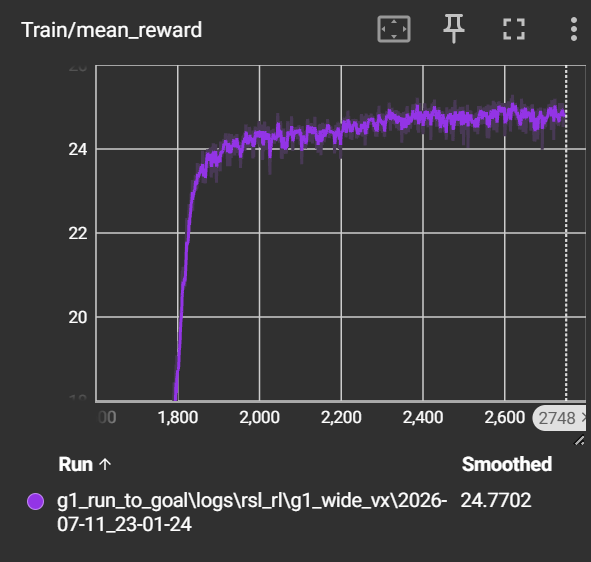
\includegraphics[width=\linewidth]{figures/tb_g1_wide_vx_mean_reward.png}
\caption*{Mean reward.}
\end{subfigure}
\hfill
\begin{subfigure}[t]{0.66\textwidth}
\centering
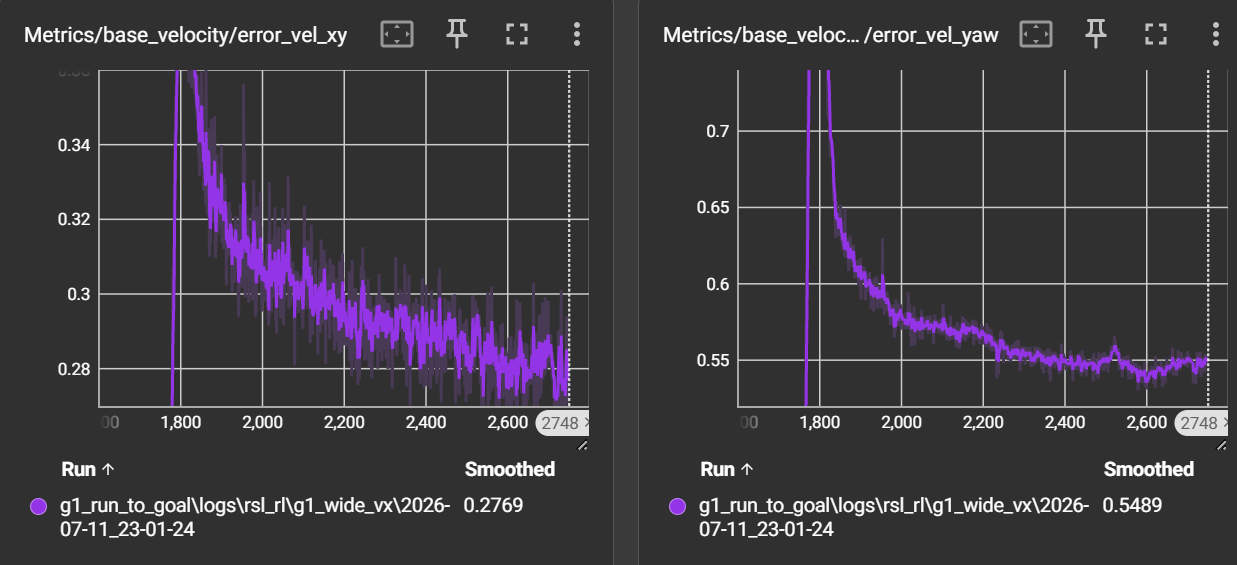
\includegraphics[width=\linewidth]{figures/tb_g1_wide_vx_metrics_error.png}
\caption*{Velocity tracking errors.}
\end{subfigure}
\caption{Wide-$v_x$ fine-tuning curves.}
\label{fig:tb-wide}
\end{figure}

\subsection{Evaluation protocol}

Both policies receive fixed, pure-forward commands
$\mathbf{c}=(v_x,0,0)$. The sweep covers $0.2$ to $2.0\,\mathrm{m/s}$; commands
through $1.0\,\mathrm{m/s}$ are in-distribution for the base policy, while
commands from $1.1$ to $2.0\,\mathrm{m/s}$ are out-of-distribution. Automatic
heading commands and standing environments are disabled so that the commanded
forward speed is the only test variable.

I record a simulation clip at each speed and compare whether the robot remains
upright and follows the command.

\subsection{Observed outcome}

In the recorded sweep, the base policy remains upright at
$v_x=1.3\,\mathrm{m/s}$ but falls at $1.4\,\mathrm{m/s}$ and at the higher
tested commands. After fine-tuning, the wide-$v_x$ policy remains upright and
follows the forward command through $2.0\,\mathrm{m/s}$. Fine-tuning therefore
extends the tested command range beyond that of the base policy.

\begin{figure}[H]
\centering
\begin{subfigure}[t]{0.48\textwidth}
\centering
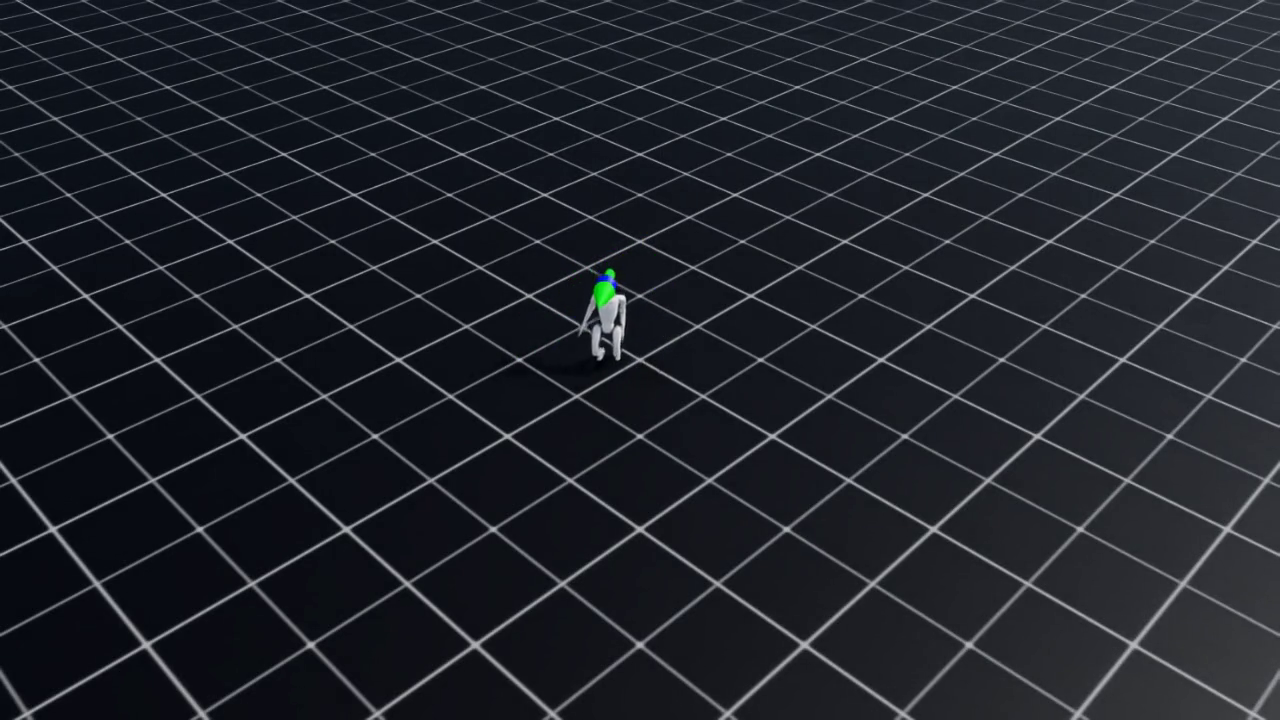
\includegraphics[width=\linewidth]{figures/fig_ood13.png}
\caption*{Base, $v_x{=}1.3\,\mathrm{m/s}$ (stable).}
\end{subfigure}
\hfill
\begin{subfigure}[t]{0.48\textwidth}
\centering
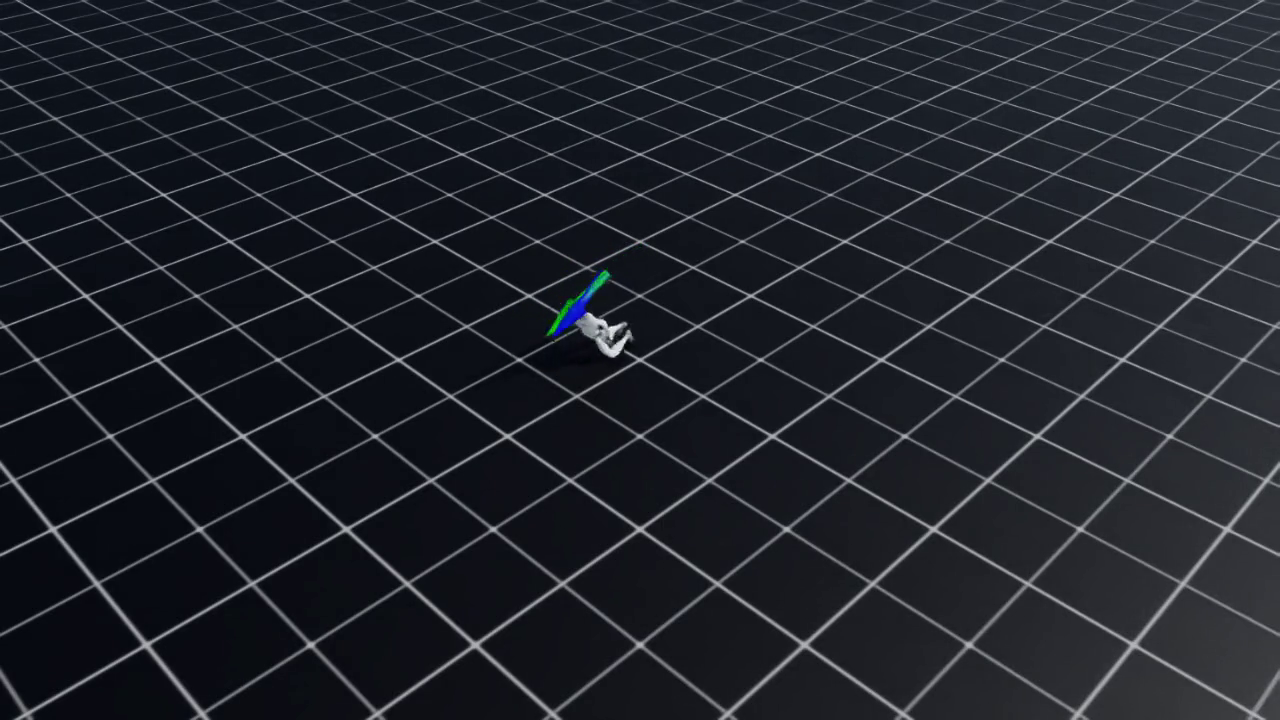
\includegraphics[width=\linewidth]{figures/fig_ood14.png}
\caption*{Base, $v_x{=}1.4\,\mathrm{m/s}$ (falls).}
\end{subfigure}

\vspace{0.6em}

\begin{subfigure}[t]{0.48\textwidth}
\centering
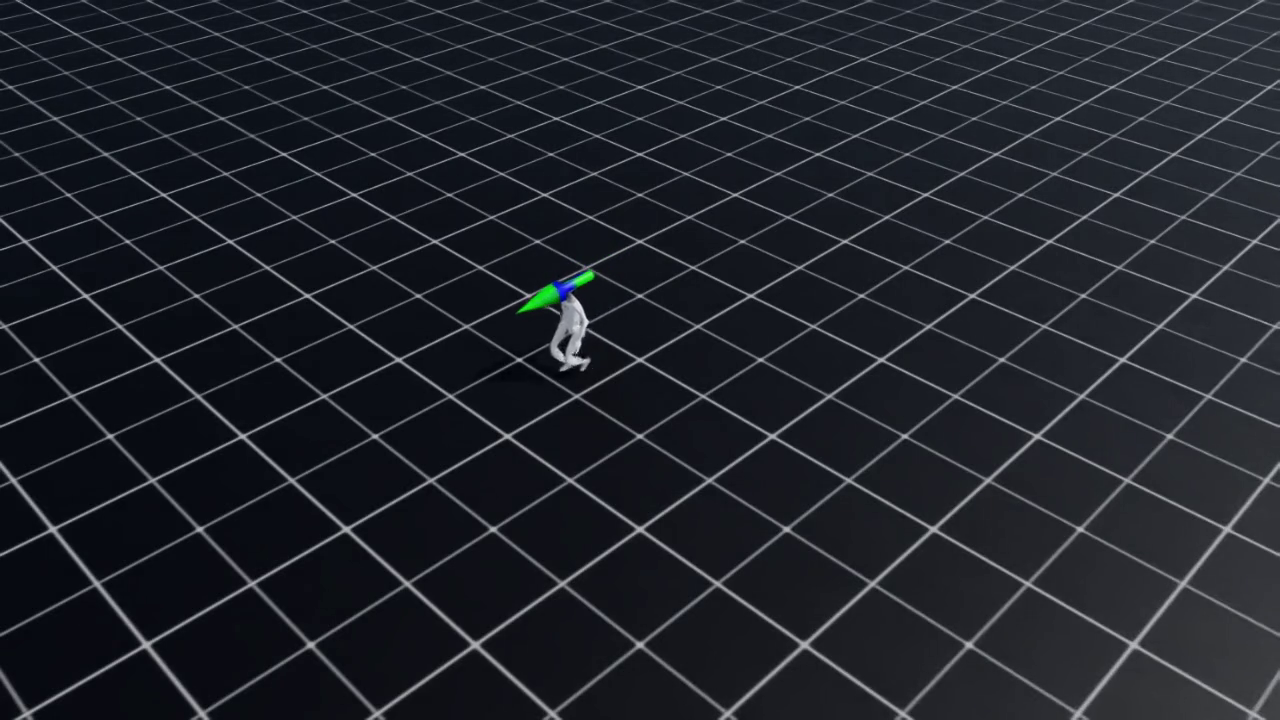
\includegraphics[width=\linewidth]{figures/fig_wide14.png}
\caption*{Wide-$v_x$, $v_x{=}1.4\,\mathrm{m/s}$.}
\end{subfigure}
\hfill
\begin{subfigure}[t]{0.48\textwidth}
\centering
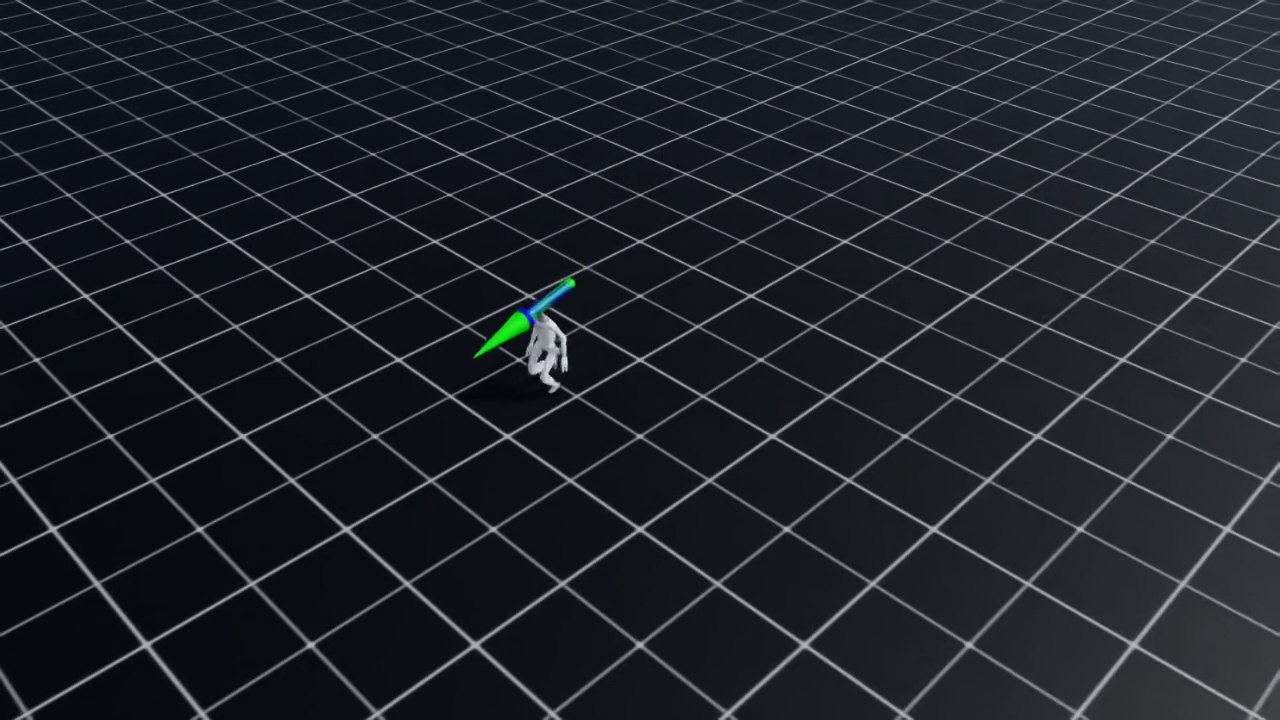
\includegraphics[width=\linewidth]{figures/fig_wide20.png}
\caption*{Wide-$v_x$, $v_x{=}2.0\,\mathrm{m/s}$.}
\end{subfigure}
\caption{OOD forward-speed frames. The base policy holds at $v_x{=}1.3\,\mathrm{m/s}$ but collapses at $v_x{=}1.4\,\mathrm{m/s}$; wide-$v_x$ recovers at $v_x{=}1.4\,\mathrm{m/s}$ and still walks at $v_x{=}2.0\,\mathrm{m/s}$.}
\label{fig:ood}
\end{figure}

\section{Exploratory Experiment II: Rough-Terrain Fine-Tuning}
\label{sec:rough}

This experiment asks whether the flat G1 velocity policy can transfer to uneven
ground \textbf{without} changing the observation dimension, so that its
pretrained weights remain compatible.

\subsection{Motivation}

Official rough terrains (stairs, random boxes, height noise, slopes) usually
come with a height scanner in the policy observation.
The flat policy has no height scan ($123$-D).
Enabling the scanner would change the network input size, so the pretrained
checkpoint could no longer be loaded.
Can I fine-tune on rough \textbf{physics} with the height scan left off and
still get usable walking?

\subsection{Setup}

\begin{table}[H]
\centering
\small
\begin{tabular}{@{}ll@{}}
\toprule
Item & Choice \\
\midrule
Terrain & \texttt{ROUGH\_TERRAINS\_CFG} + curriculum from level 0 \\
Observations & Same as flat: no \texttt{height\_scan} \\
Initialization & Base flat velocity policy (not the wide-$v_x$ policy) \\
Commands & $v_x\in[0,2]$, $v_y\in[-0.5,0.5]$, $\omega_z\in[-1,1]$ \\
Rewards & Official G1 rough; \texttt{lin\_vel\_z\_l2}${}=0$ \\
Envs & 4096 \\
\bottomrule
\end{tabular}
\caption{Rough-terrain fine-tuning setup.}
\label{tab:rough}
\end{table}

The fine-tune starts from the base flat policy, so it widens the forward
command range to $[0,2]\,\mathrm{m/s}$ and changes the terrain at the same
time. The vertical-velocity penalty \texttt{lin\_vel\_z\_l2} is set to zero
because stepping up and down stairs requires vertical base motion that the
flat reward would punish.

\subsection{Training}

The flat policy is fine-tuned on rough terrain for 351 iterations.
Figure~\ref{fig:tb-rough} shows the mean episode length rising and holding near $850$ control steps, while the terrain curriculum climbs from level~$1$ toward about $3.4$.

\begin{figure}[H]
\centering
\begin{subfigure}[t]{0.48\textwidth}
\centering
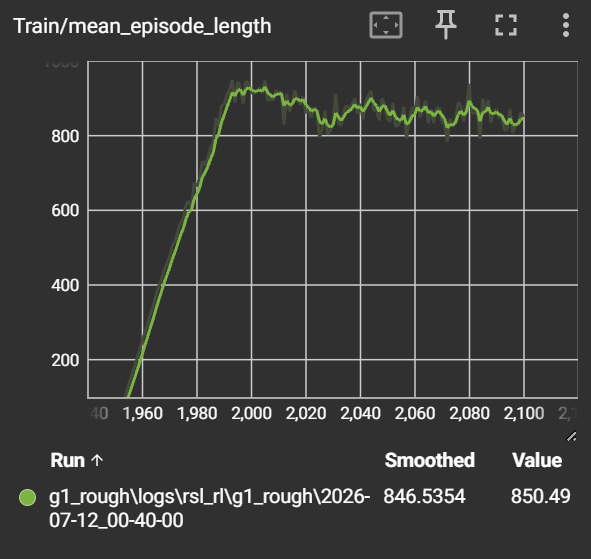
\includegraphics[width=\linewidth]{figures/tb_g1_rough_eps_length.png}
\caption*{Mean episode length.}
\end{subfigure}
\hfill
\begin{subfigure}[t]{0.48\textwidth}
\centering
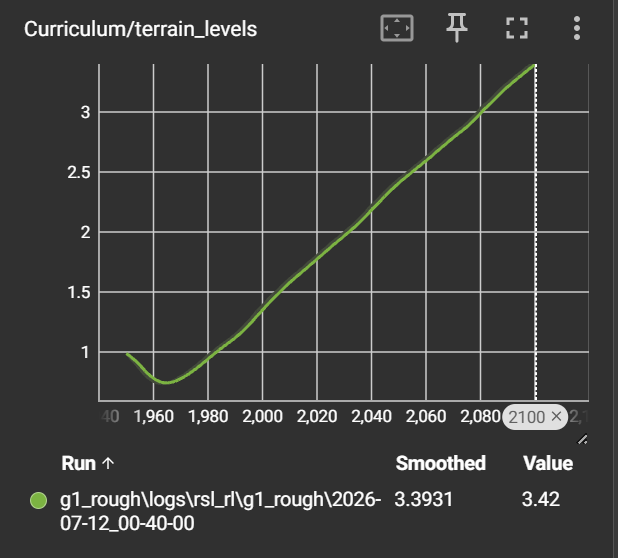
\includegraphics[width=\linewidth]{figures/tb_g1_rough_terrain_levels.png}
\caption*{Terrain curriculum level.}
\end{subfigure}
\caption{Rough-terrain fine-tuning: episode length and curriculum progress.}
\label{fig:tb-rough}
\end{figure}

\subsection{Outcome}

After fine-tuning, the policy can walk over stairs, random
boxes, slopes, and height noise without a height scan. It still falls on some
of the harder tiles because it cannot see the terrain ahead and must react
after contact. More training would probably help, but the GPU had other
appointments on its calendar.

\begin{figure}[H]
\centering
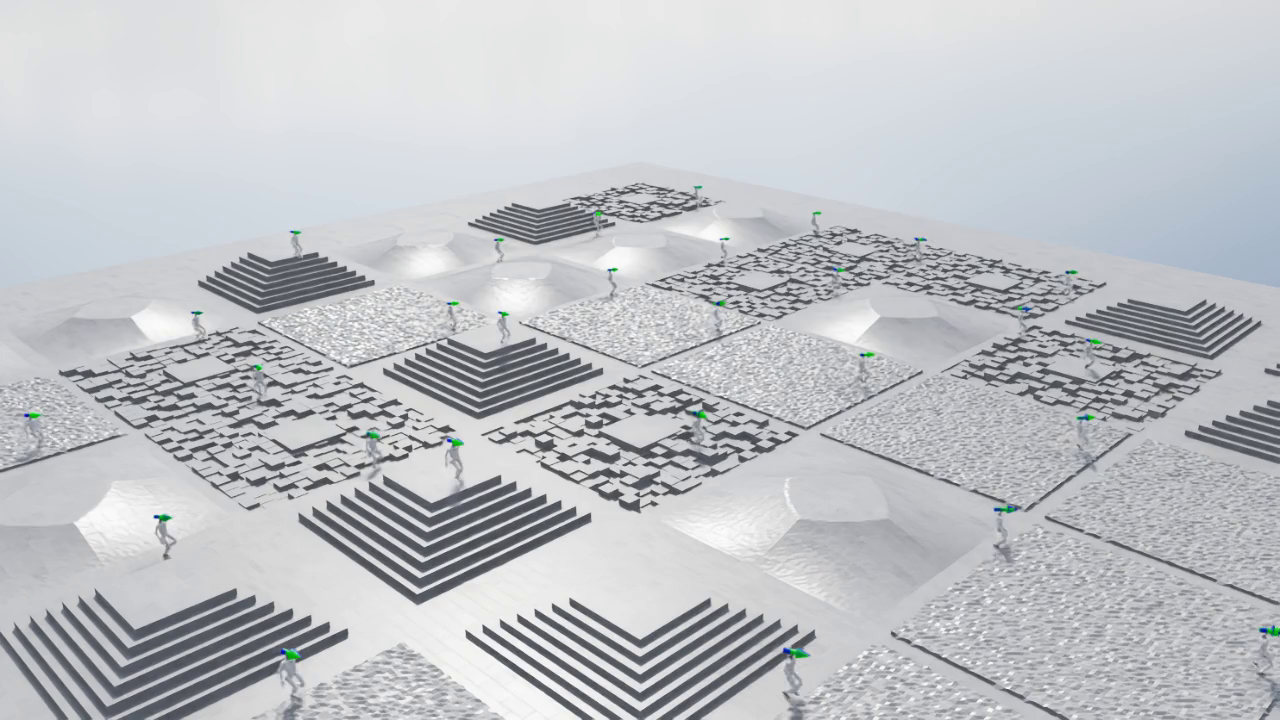
\includegraphics[width=0.92\textwidth]{figures/fig_rough.png}
\caption{Rough-terrain demo after fine-tuning. The policy navigates stairs,
random boxes, height noise, and slopes without a height scan.}
\label{fig:rough}
\end{figure}

\section{Summary}
\label{sec:summary}

The main takeaway is that a velocity policy can be reused for goal tracking:
a simple proportional controller generates velocity commands, while the
learned policy handles walking. The experiments also show that the training
distribution matters. Fine-tuning extends the tested forward speed from
$1.3\,\mathrm{m/s}$ to $2.0\,\mathrm{m/s}$ and allows the flat policy to walk
on rough terrain without changing its observation size.

The main limitations are that the speed and rough-terrain results are based on
qualitative videos rather than repeated trials or numerical benchmarks. The
rough policy is fine-tuned only briefly and has no height scan, so
it cannot see upcoming terrain. I evaluate the policy only in simulation.

\bibliographystyle{plainnat}
\bibliography{ref}
\end{document}
